\clearpage
\section{Exercises Part 1}

\subsection{Exercise 1.1: Sorting Complexity}
\textbf{Problem:} A sorting method with “Big-Oh” complexity $O(n \log n)$ spends exactly 1 millisecond to sort 1,000 data items. Given this, estimate how long it will take to sort 1,000,000 items.

\vspace{0.5em}
\textbf{Solution Steps:}
\begin{enumerate}[leftmargin=*,noitemsep]
    \item Understand the Problem: You need to find out how long it will take to sort 1,000,000 items using the given complexity.
    \item Identify Known Values:
    \begin{itemize}
        \item $T(1,000) = 1ms$
        \item Complexity is $O(n \log n)$
    \end{itemize}
    \item Calculate Constant $c$:
    \begin{itemize}
        \item Formula: $T(n) = c \cdot n \log n$
        \item Use $T(1,000) = 1ms$ to find $c$:
        \[ c = \frac{1ms}{1,000 \log 1,000} \]
    \end{itemize}
    \item Calculate $T(1,000,000)$:
    \begin{itemize}
        \item Use the formula $T(n) = c \cdot n \log n$
        \item Substitute $n = 1,000,000$:
        \[ T(1,000,000) = c \cdot 1,000,000 \cdot \log 1,000,000 \]
    \end{itemize}
    \item Simplify the Expression:
    \begin{itemize}
        \item Calculate $\log 1,000,000$
        \item Multiply and simplify to find the time in seconds.
    \end{itemize}
\end{enumerate}

\textbf{Exam Note:} Remember that $O(n \log n)$ complexity means the time increases logarithmically with the size of the data.

\textbf{Hint:} To solve similar exercises, focus on understanding the relationship between the given complexity and the time it takes to process a certain amount of data. Use the formula $T(n) = c \cdot f(n)$ to calculate the constant $c$ and then use it to find the time for a different amount of data.

\subsection{Exercise 1.2: Quadratic Algorithm}
\textbf{Problem:} A quadratic algorithm with processing time $T(n) = cn^2$ spends 1ms for 100 items. Calculate the time for 5,000 items.

\vspace{0.5em}
\textbf{Solution Steps:}
\begin{enumerate}[leftmargin=*,noitemsep]
    \item Understand the Problem: You need to calculate the time for 5,000 items given the complexity.
    \item Identify Known Values:
    \begin{itemize}
        \item $T(100) = 1ms$
        \item Complexity is $O(n^2)$
    \end{itemize}
    \item Calculate Constant $c$:
    \begin{itemize}
        \item Formula: $T(n) = c \cdot n^2$
        \item Use $T(100) = 1ms$ to find $c$:
        \[ c = \frac{1ms}{100^2} \]
    \end{itemize}
    \item Calculate $T(5,000)$:
    \begin{itemize}
        \item Use the formula $T(n) = c \cdot n^2$
        \item Substitute $n = 5,000$:
        \[ T(5,000) = c \cdot (5,000)^2 \]
    \end{itemize}
    \item Simplify the Expression:
    \begin{itemize}
        \item Calculate $(5,000)^2$
        \item Multiply and simplify to find the time in milliseconds.
    \end{itemize}
\end{enumerate}

\textbf{Exam Note:} Quadratic complexity $O(n^2)$ means time increases with the square of the data size.

\textbf{Hint:} To solve similar exercises, focus on understanding the relationship between the given complexity and the time it takes to process a certain amount of data. Use the formula $T(n) = c \cdot f(n)$ to calculate the constant $c$ and then use it to find the time for a different amount of data.

\subsection{Exercise 1.3: Time Complexity}
\textbf{Problem:} Given $T(n) = c \cdot f(n)$, where $f(n) = n$ or $f(n) = n^3$, calculate the time for 100,000 items.

\vspace{0.5em}
\textbf{Solution Steps:}
\begin{enumerate}[leftmargin=*,noitemsep]
    \item Understand the Problem: You need to calculate the time for different functions $f(n)$.
    \item Identify Known Values:
    \begin{itemize}
        \item $T(1,000) = 10s$
        \item Functions $f(n) = n$ and $f(n) = n^3$
    \end{itemize}
    \item Calculate Constant $c$ for Each Function:
    \begin{itemize}
        \item Use $T(1,000) = 10s$ to find $c$ for each $f(n)$.
    \end{itemize}
    \item Calculate $T(100,000)$ for Each Function:
    \begin{itemize}
        \item For $f(n) = n$, compute $T(100,000)$.
        \item For $f(n) = n^3$, compute $T(100,000)$.
    \end{itemize}
    \item Simplify the Expressions:
    \begin{itemize}
        \item Calculate the necessary values and simplify.
    \end{itemize}
\end{enumerate}

\textbf{Exam Note:} Understand how different functions $f(n)$ affect time complexity.

\textbf{Hint:} To solve similar exercises, focus on understanding the relationship between the given complexity and the time it takes to process a certain amount of data. Use the formula $T(n) = c \cdot f(n)$ to calculate the constant $c$ and then use it to find the time for a different amount of data.

\subsection{Exercise 1.4: Dominant Terms}
\textbf{Problem:} Analyze expressions to find dominant terms and Big-Oh complexity.

\vspace{0.5em}
\textbf{Solution Steps:}
\begin{enumerate}[leftmargin=*,noitemsep]
    \item Understand the Problem: You need to identify the dominant term in each expression.
    \item Analyze Each Expression:
    \begin{itemize}
        \item Look for the term that grows fastest as $n$ increases.
        \item Example: For the expression $5n^2 + 3n \log n$, the term $5n^2$ grows faster than $3n \log n$.
    \end{itemize}
    \item Determine Big-Oh Notation:
    \begin{itemize}
        \item Use the dominant term to find the Big-Oh notation.
        \item Example: $5n^2 + 3n \log n$ is $O(n^2)$.
    \end{itemize}
    \item Practice with Examples:
    \begin{itemize}
        \item Expression: $n^3 + n^2 \log n$
        \item Dominant Term: $n^3$
        \item Big-Oh: $O(n^3)$
    \end{itemize}
\end{enumerate}

\textbf{Exam Note:} Focus on the term that grows fastest as $n$ increases.

\textbf{Hint:} To solve similar exercises, focus on identifying the dominant term in each expression. Use the properties of logarithms and powers of $n$ to analyze the relationships between terms and determine the Big-Oh notation.

\begin{table}[h]
    \centering
    \small
    \begin{tabularx}{\linewidth}{|X|X|X|}
        \hline
        Expression & Dominant term(s) & $O(\ldots)$ \\
        \hline
        5 + 0.001$n^3$ + 0.025$n$ & 0.001$n^3$ & $O(n^3)$ \\
        \hline
        500$n$ + 100$n^{1.5}$ + 50$n \log_{10} n$ & 100$n^{1.5}$ & $O(n^{1.5})$ \\
        \hline
        0.3$n$ + 5$n^{1.5}$ + 2.5 $\cdot$ $n^{1.75}$ & 2.5$n^{1.75}$ & $O(n^{1.75})$ \\
        \hline
        $n^2 \log_2 n$ + $n(n \log n)^2$ & $n^2 \log n$ & $O(n^2 \log n)$ \\
        \hline
        $n \log_3 n$ + $n \log_2 n$ & $n \log_3 n, n \log_2 n$ & $O(n \log n)$ \\
        \hline
        3 $\log_8 n$ + $\log_2 \log_2 \log_2 n$ & 3 $\log_8 n$ & $O(\log n)$ \\
        \hline
        100$n$ + 0.01$n^2$ & 0.01$n^2$ & $O(n^2)$ \\
        \hline
        0.01$n$ + 100$n^2$ & 100$n^2$ & $O(n^2)$ \\
        \hline
        2$n$ + $n^{0.5}$ + 0.5$n^{1.25}$ & 0.5$n^{1.25}$ & $O(n^{1.25})$ \\
        \hline
        0.01$n \log_2 n$ + $n(\log_2 n)^2$ & $n(\log_2 n)^2$ & $O(n(\log n)^2)$ \\
        \hline
        100$n \log_3 n$ + $n^3$ + 100$n$ & $n^3$ & $O(n^3)$ \\
        \hline
        0.003 $\log_4 n$ + $\log_2 \log_2 n$ & 0.003 $\log_4 n$ & $O(\log n)$ \\
        \hline
    \end{tabularx}
    \caption{Dominant terms and Big-Oh notation for various expressions.}
\end{table}

\textbf{Exam Note:} Focus on the term that grows fastest as $n$ increases.

\textbf{Hint:} To solve similar exercises, focus on identifying the dominant term in each expression. Use the properties of logarithms and powers of $n$ to analyze the relationships between terms and determine the Big-Oh notation.

\subsection{Exercise 1.5: Big-Oh Notation}
\textbf{Problem:} Determine if statements about Big-Oh notation are true or false.

\vspace{0.5em}
\textbf{Solution Steps:}
\begin{enumerate}[leftmargin=*,noitemsep]
    \item Understand the Problem: You need to evaluate the truth of each statement about Big-Oh notation.
    \item Evaluate Each Statement:
    \begin{itemize}
        \item Rule of Sums: $O(f + g) = O(\max\{f, g\})$
        \item Rule of Products: $O(f \cdot g) = O(f) \cdot O(g)$
        \item Transitivity: If $g = O(f)$ and $h = O(g)$, then $h = O(f)$
    \end{itemize}
    \item Correct Any False Statements:
    \begin{itemize}
        \item If a statement is false, provide the correct formula.
        \item Example: If $O(f + g) = O(f) + O(g)$ is false, correct it to $O(f + g) = O(\max\{f, g\})$
    \end{itemize}
\end{enumerate}

\textbf{Exam Note:} Understand the properties of Big-Oh notation and be able to apply them to different scenarios.

\textbf{Hint:} To solve similar exercises, focus on understanding the properties of Big-Oh notation. Use the rules of sums, products, and transitivity to evaluate the truth of each statement.

\begin{table}[h]
    \centering
    \small
    \begin{tabularx}{\linewidth}{|X|X|X|}
        \hline
        Statement & Is it TRUE or FALSE? & If it is FALSE then write the correct formula \\
        \hline
        Rule of sums: $O(f + g) = O(f) + O(g)$ & FALSE & $O(f + g) = \max\{O(f), O(g)\}$ \\
        \hline
        Rule of products: $O(f \cdot g) = O(f) \cdot O(g)$ & TRUE & \\
        \hline
        Transitivity: if $g = O(f)$ and $h = O(f)$ then $g = O(h)$ & FALSE & if $g = O(f)$ and $f = O(h)$ then $g = O(h)$ \\
        \hline
        $5n + 8n^2 + 100n^3 = O(n^4)$ & TRUE & \\
        \hline
        $5n + 8n^2 + 100n^3 = O(n^2 \log n)$ & FALSE & $5n + 8n^2 + 100n^3 = O(n^3)$ \\
        \hline
    \end{tabularx}
    \caption{Evaluation of Big-Oh notation statements.}
\end{table}

\textbf{Exam Note:} Understand the properties of Big-Oh notation and be able to apply them to different scenarios.

\textbf{Hint:} To solve similar exercises, focus on understanding the properties of Big-Oh notation. Use the rules of sums, products, and transitivity to evaluate the truth of each statement.

\subsection{Exercise 1.6: Computational Complexity}
\textbf{Problem:} Analyze the complexity of a given algorithm.

\vspace{0.5em}
\textbf{Solution Steps:}
\begin{enumerate}[leftmargin=*,noitemsep]
    \item Understand the Problem: You need to break down the algorithm to find its complexity.
    \item Analyze Each Loop:
    \begin{itemize}
        \item Identify the number of iterations for each loop.
        \item Example: For a loop running from 1 to $n$, the complexity is $O(n)$.
    \end{itemize}
    \item Combine Results for Total Complexity:
    \begin{itemize}
        \item Multiply the complexities of nested loops.
        \item Example: A loop inside another loop, both running $n$ times, results in $O(n^2)$.
    \end{itemize}
    \item Simplify the Total Complexity:
    \begin{itemize}
        \item Combine terms to find the overall complexity.
        \item Example: If you have $O(n^2) + O(n)$, the dominant term is $O(n^2)$.
    \end{itemize}
\end{enumerate}

\textbf{Exam Note:} Pay close attention to nested loops and their impact on complexity. Practice breaking down algorithms into their basic components to understand their efficiency.

\textbf{Hint:} To solve similar exercises, focus on breaking down the algorithm into its basic components. Analyze each loop and combine the results to find the total complexity.

\FloatBarrier

\subsection{Exercise 2: Binary Search Tree Property}

\textbf{Problem:} Consider a binary search tree $T$ whose keys are distinct. Show that if the right subtree of a node $x$ in $T$ is empty and $x$ has a successor $y$, then $y$ is the lowest ancestor of $x$ whose left child is also an ancestor of $x$. (Recall that every node is its own ancestor.)

\textbf{Solution:} Let's prove this by contradiction:

\begin{enumerate}
    \item First, observe that since $x$ has no right subtree, its successor $y$ must be an ancestor of $x$.
        \begin{itemize}
            \item This is because in a BST, if $x$ had any right child, its successor would be in that subtree.
            \item Since there is no right subtree, we must go up the tree to find a larger value.
        \end{itemize}
    
    \item Assume for contradiction that there exists a node $z \neq y$ that is:
        \begin{itemize}
            \item The lowest ancestor of $x$ whose left child is an ancestor of $x$
            \item Different from $y$ (the successor of $x$)
        \end{itemize}
\end{enumerate}

\begin{figure}[H]
    \centering
    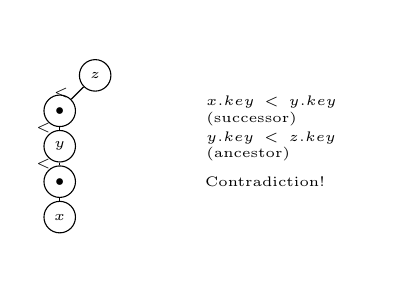
\begin{tikzpicture}[scale=0.45,
        level distance=1cm,
        level 1/.style={sibling distance=2cm},
        level 2/.style={sibling distance=1cm},
        every node/.style={circle,draw,inner sep=1pt,font=\tiny,minimum size=0.4cm}]
        
        % The tree showing contradiction
        \node (z) {$z$}
            child {
                node (leftz) {$\bullet$}
                child {
                    node (y) {$y$} 
                    child {
                        node (lefty) {$\bullet$}
                        child {
                            node (x) {$x$}
                        }
                        edge from parent node[left,draw=none,font=\tiny] {$<$}
                    }
                    edge from parent node[left,draw=none,font=\tiny] {$<$}
                }
                edge from parent node[left,draw=none,font=\tiny] {$<$}
            }
            child[missing];
            
        % Add explanatory text
        \node[draw=none,font=\tiny,text width=2cm,anchor=west] at (3,-1) 
            {$x.key < y.key$ (successor)};
        \node[draw=none,font=\tiny,text width=2cm,anchor=west] at (3,-2) 
            {$y.key < z.key$ (ancestor)};
        \node[draw=none,font=\tiny,text width=2cm,anchor=west] at (3,-3) 
            {Contradiction!};
    \end{tikzpicture}
    \caption*{\footnotesize Contradiction in BST property}
\end{figure}

This leads to a contradiction because:
\begin{itemize}
    \item Since $x$ is in the left subtree of $y$: $x.key < y.key$
    \item Since $z$ is an ancestor of $y$: $y.key < z.key$
    \item But $y$ is the successor of $x$, so there can't be any value $z.key$ between $x.key$ and $y.key$
    \item Therefore, $z$ must be $y$
\end{itemize}

Thus, $y$ (the successor of $x$) must be the lowest ancestor of $x$ whose left child is also an ancestor of $x$.

\subsection{Exercise 2.1: Heap Structure}
\textbf{Problem:} Viewing a heap as a tree, we define the height of a node in a heap to be the number of edges on the longest simple downward path from the node to a leaf, and we define the height of the heap to be the height of its root. What are the minimum and maximum numbers of elements in a heap of height $h$?

\vspace{0.5em}
\textbf{Solution:} From the previous exercise (in particular its solution) we have seen that

\[ 2^h \leq n \leq 2^{h+1} - 1 \]

where $h$ is the height of the complete binary tree. By taking the logarithm $\lg$ in base 2 at each term of the above sequence of inequalities, since $\lg$ is a monotone increasing function we have

\[ h \leq \ln n \leq \ln(2^{h+1} - 1) \]

Now it is enough to note that

\[ h = \ln 2^h \leq \ln n \leq \ln(2^{h+1} - 1) < h + 1 \]

Thus we have

\[ h = \lfloor h \rfloor \leq \lfloor \ln n \rfloor \leq \lfloor \ln(2^{h+1} - 1) \rfloor = h \]

\begin{figure}[H]
    \centering
    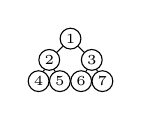
\begin{tikzpicture}[scale=0.45,
        level distance=0.6cm,
        level 1/.style={sibling distance=1.2cm},
        level 2/.style={sibling distance=0.6cm},
        every node/.style={circle,draw,inner sep=1pt,font=\tiny}]
        \node {1}
            child {node {2}
                child {node {4}}
                child {node {5}}
            }
            child {node {3}
                child {node {6}}
                child {node {7}}
            };
    \end{tikzpicture}
    \caption*{\footnotesize Simple Binary Tree Representing a Heap}
\end{figure}

\textbf{Hint:} To solve similar exercises, focus on understanding the structure of heaps and binary trees. Use the properties of logarithms and powers of 2 to analyze the relationships between nodes and height.

\subsection{Exercise 2.2: Heap Height}
\textbf{Problem:} Show that an $n$-element heap has height $\lfloor \lg n \rfloor$. (Where $\lg(\cdot)$ denotes logarithm in base 2).

\vspace{0.5em}
\textbf{Solution:} From the previous exercise (in particular its solution) we have seen that

\[ 2^h \leq n \leq 2^{h+1} - 1 \]

where $h$ is the height of the complete binary tree. By taking the logarithm $\lg$ in base 2 at each term of the above sequence of inequalities, since $\lg$ is a monotone increasing function we have

\[ h \leq \ln n \leq \ln(2^{h+1} - 1) \]

Now it is enough to note that

\[ h = \ln 2^h \leq \ln n \leq \ln(2^{h+1} - 1) < h + 1 \]

Thus we have

\[ h = \lfloor h \rfloor \leq \lfloor \ln n \rfloor \leq \lfloor \ln(2^{h+1} - 1) \rfloor = h \]

\textbf{Hint:} To solve similar exercises, focus on understanding the structure of heaps and binary trees. Use the properties of logarithms and powers of 2 to analyze the relationships between nodes and height.

\subsection{Exercise 2.4: Recursive Algorithm Running Time}
\textbf{Problem:} We consider the running time of a recursive algorithm $y(n)$. Suppose that $y(n)$ verifies the following:

1. \[
\begin{cases}
    y(1) = 0 \\
    y(n) = y\left(\frac{n}{2}\right) + 1 & n \geq 1
\end{cases}
\]
If possible, calculate the running time.

2. \[
\begin{cases}
    y(1) = 0 \\
    y(n) = 3y\left(\frac{n}{4}\right) + n^2 \log_2 n & n \geq 1
\end{cases}
\]
If possible, calculate the running time.

3. \[
\begin{cases}
    y(1) = 0 \\
    y(n) = 5y\left(\frac{n}{3}\right) + \log_2 n & n \geq 1
\end{cases}
\]
If possible, calculate the running time.

\vspace{0.5em}
\textbf{Solution:} Using the Master Theorem:

1. We have $a = 1$, $b = 2$, and $f(n) = 1$. Since $n^{\log_b a} = n^0 = 1$, we have $f(n) = \Theta(1)$. Thus we are in case II of the Master Theorem. So $T(n) = \Theta(\ln n)$.

2. We have $a = 3$, $b = 4$, and $f(n) = n^2 \log_2 n$. Since $n^{\log_b a} = n^{\log_4 3}$, we have $f(n) = \Omega(n^{\log_4 3 + \epsilon})$ for some $\epsilon > 0$. Therefore, for the Master Theorem (case 3), we have $T(n) = \Theta(n^2 \ln n)$.

3. We have $a = 5$, $b = 3$, and $f(n) = \log_2 n$. Since $n^{\log_b a} = n^{\log_3 5} > n$, we have $f(n) = O(n^{\log_3 5 - \epsilon})$ for some $\epsilon > 0$. Therefore, we are in case 1 of the Master Theorem, and so $T(n) = \Theta(n^{\log_3 5})$. 

\textbf{Conclusion:} To apply the Master Theorem, follow these steps:

1. Identify the parameters $a$, $b$, and $f(n)$ from the recurrence relation.
2. Calculate $n^{\log_b a}$ to compare with $f(n)$.
3. Determine which case of the Master Theorem applies:
   - \textbf{Case 1:} If $f(n)$ grows slower than $n^{\log_b a}$, then $T(n) = \Theta(n^{\log_b a})$.
   - \textbf{Case 2:} If $f(n)$ grows at the same rate as $n^{\log_b a}$, then $T(n) = \Theta(n^{\log_b a} \log n)$.
   - \textbf{Case 3:} If $f(n)$ grows faster than $n^{\log_b a}$, then check the regularity condition. If it holds, $T(n) = \Theta(f(n))$.

This approach helps in determining the asymptotic behavior of recursive algorithms efficiently.

\textbf{Hint:} To solve similar exercises, identify the parameters $a$, $b$, and $f(n)$ in the recurrence relation, and apply the Master Theorem to determine the running time.

\subsection{Exercise 3.1: HEAPSORT Operations}
\textbf{Problem:} Using the figure in slide 25 of the slide of week 2 as a model, illustrate the operations of HEAPSORT on the array

\[ A = \{5, 13, 2, 25, 7, 17, 20, 8, 4\} \]

\vspace{0.5em}
\textbf{Solution:} Let's break down the HEAPSORT process into detailed steps:

1. \textbf{Build Max-Heap (BUILD-MAX-HEAP)}:
   \begin{itemize}
      \item Start with the array as a binary tree (parent at $i$, children at $2i$ and $2i+1$)
      \item For each non-leaf node from $\lfloor n/2 \rfloor$ down to 1:
         \begin{itemize}
            \item Call MAX-HEAPIFY on that node
            \item This ensures the subtree rooted at each node satisfies max-heap property
         \end{itemize}
   \end{itemize}

2. \textbf{Extract and Sort (HEAPSORT)}:
   \begin{itemize}
      \item For $i$ from $n$ down to 2:
         \begin{itemize}
            \item Swap $A[1]$ (root) with $A[i]$ (last element)
            \item Reduce heap size by 1
            \item Call MAX-HEAPIFY on root (1) to maintain max-heap property
         \end{itemize}
   \end{itemize}

\textbf{Detailed Process for Our Array}:
\begin{enumerate}[label=\arabic*.]
    \item Initial array: $\{5, 13, 2, 25, 7, 17, 20, 8, 4\}$
    \item BUILD-MAX-HEAP:
       \begin{itemize}
          \item Start from last non-leaf node ($\lfloor 9/2 \rfloor = 4$)
          \item Apply MAX-HEAPIFY at each level up to root
          \item Results in max-heap with 25 at root
       \end{itemize}
    \item HEAPSORT Process:
       \begin{itemize}
          \item Swap 25 with last element, heapify remaining
          \item Swap new max with second-to-last, heapify
          \item Continue until all elements processed
       \end{itemize}
    \item Final sorted array: $\{2, 4, 5, 7, 8, 13, 17, 20, 25\}$
\end{enumerate}

\textbf{Key Operations}:
\begin{itemize}
    \item MAX-HEAPIFY($A,i$): Ensures subtree at index $i$ maintains max-heap property
    \item BUILD-MAX-HEAP($A$): Converts array into max-heap
    \item HEAPSORT($A$): Repeatedly extracts maximum and rebuilds heap
\end{itemize}

\begin{figure}[H]
    \centering
    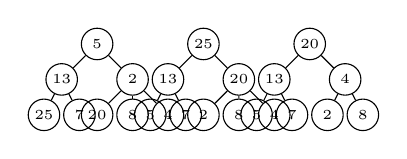
\begin{tikzpicture}[scale=0.45,
        level distance=1cm,
        level 1/.style={sibling distance=2cm},
        level 2/.style={sibling distance=1cm},
        level 3/.style={sibling distance=0.8cm},
        every node/.style={circle,draw,inner sep=1pt,font=\tiny,minimum size=0.4cm}]
        
        % Initial tree
        \node {5}
            child {node {13}
                child {node {25}}
                child {node {7}}
            }
            child {node {2}
                child {node {20}}
                child {node {8}}
                child {node {4}}
            };
            
        % After BUILD-MAX-HEAP
        \begin{scope}[xshift=3cm]
        \node {25}
            child {node {13}
                child {node {5}}
                child {node {7}}
            }
            child {node {20}
                child {node {2}}
                child {node {8}}
                child {node {4}}
            };
        \end{scope}
        
        % After first extraction
        \begin{scope}[xshift=6cm]
        \node {20}
            child {node {13}
                child {node {5}}
                child {node {7}}
            }
            child {node {4}
                child {node {2}}
                child {node {8}}
            };
        \end{scope}
    \end{tikzpicture}
    \caption*{\footnotesize HEAPSORT steps: Initial $\rightarrow$ BUILD-MAX-HEAP $\rightarrow$ First extraction}
\end{figure}

\textbf{Note:} The process continues similarly until all elements are sorted. At each step:
\begin{itemize}
    \item The largest element moves to the root
    \item We swap it with the last element of the current heap
    \item We reduce the heap size and MAX-HEAPIFY the root
\end{itemize}

\textbf{Hint:} To solve similar exercises:
\begin{enumerate}
    \item Draw the initial array as a complete binary tree
    \item Apply BUILD-MAX-HEAP by working bottom-up
    \item For each HEAPSORT step:
       \begin{itemize}
          \item Draw the current heap state
          \item Show the swap operation
          \item Show the heapified result
       \end{itemize}
    \item Keep track of the sorted portion at the end of the array
\end{enumerate}
